\documentclass[xcolor=pdftex,dvipsnames,table]{beamer}


\mode<presentation> {
  \usetheme{Warsaw}
  \setbeamercovered{transparent}
%  \useoutertheme{infolines}
%  \setbeamertemplate{headline}[default]
%  \setbeamertemplate{footline}[infolines theme]{}
}

\usepackage[english]{babel}

\usepackage[latin1]{inputenc}

\usepackage{times}
\usepackage[T1]{fontenc}

\usepackage{ulem}
\usepackage{amssymb}

\hypersetup{%
    pdftitle={Performance Modelling of Peer-to-Peer Routing},
    pdfauthor={Idris A. Rai, Andrew Brampton, Andrew MacQuire, and Laurent Mathy},
%    pdfkeywords={Distributed Hash Tables, Peer-to-Peer, Stealth DHT},
    bookmarksnumbered,
    pdfstartview={FitV},
    linkcolor={black},%: Color for normal internal links.
    anchorcolor={black},%: Color for anchor text.
    citecolor={black},%: Color for bibliographical citations in text.
    filecolor={black},%: Color for URLs which open local files.
    menucolor={black},%: Color for Acrobat menu items.
    pagecolor={black},%: Color for links to other pages
    urlcolor={black},%: Color for linked URLs.
}%

\title[Modelling Peer-to-Peer Routing]
{\textbf{Performance Modelling of Peer-to-Peer Routing}}

\institute[Lancaster University, UK] {
  \textbf{Idris A. Rai}, Andrew Brampton, Andrew MacQuire, and Laurent Mathy\\
  {\it \{rai,brampton,macquire,laurent\}@comp.lancs.ac.uk}\\
  Computing Department\\
  Lancaster University, UK
}

\date[30th March 2007]
{Friday 30 March \\ \textbf{Hot-P2P 2007}}

\subject{Modelling Peer-to-Peer Routing}

\logo{
\includegraphics[height=0.85cm]{uni-logo-win}}

\setbeamertemplate{navigation symbols}{}

%\renewcommand{\textbf}{\alert}

\begin{document}

\begin{frame}
  \titlepage
\end{frame}

\begin{frame}
  \frametitle{Outline}
%  \tableofcontents
  \begin{itemize}
  \item Motivation
     \begin{itemize}
        \item Distributed Hash Table (DHT) (Pastry)
        \item Stealth DHT
    \end{itemize}
  \item Modelling
       \begin{itemize}
        \item Markov Chains
        \item Transition probabilities
        \item Stationary Solutions
    \end{itemize}
  \item Validations
  \item Conclusion
  \end{itemize}
\end{frame}

\section{Motivation}

\subsection{Distributed Hash}
\begin{frame}
  \frametitle{Distributed Has Table Overview}
  \begin{columns}

  \column{6cm}
%    \textbf{Pastry}
     \begin{itemize}
     \item{Circular Identifier Space (typically $0-2^{128}$)}
     \item{Each node has ID\\Each key has ID}
     \item{Nodes are responsible for keys closest to them (on the ring)}
     \item{Routing done iteratively closer and closer to a ID}
     \end{itemize}
  \column{6cm}
  \begin{center}
    \begin{overlayarea}{\textwidth}{0.8\textheight}
        \includegraphics<1>[width=6cm]{diagrams/DHT}
    \end{overlayarea}
  \end{center}
  \end{columns}

\end{frame}

\begin{frame}
  \frametitle{Distributed Hash Table Problems}
  \begin{columns}

  \column{6cm}

  \begin{itemize}
    \frametitle{}
    \item<1-2>{\textbf{Assumed homogeneity}}~\\
        {Varying bandwidth, processing or storage abilities}
    \item<3>{\textbf{Churn overhead}}~\\
        {Joining causes updates, Leaving causes staleness}
    \item<4>{\textbf{Free-riding}}~\\
        {Users don't want to participate, or stay for a very short time}
    \item<5>{\textbf{Security issues}}~\\
        {Sniffing, Man in the middle, Poisoning, Denial of Service}
  \end{itemize}

  \column{6cm}

  \begin{center}
    \begin{overlayarea}{\textwidth}{0.8\textheight}
        \includegraphics<1>[width=6cm]{diagrams/DHT}
        \includegraphics<2>[width=6cm]{diagrams/Homogeneity}
        \includegraphics<3-4>[width=6cm]{diagrams/Churn}
        %AB: Maybe some kind of graphic for 4
        \includegraphics<5>[width=5.5cm]{diagrams/Security}
    \end{overlayarea}
  \end{center}
\end{columns}
\end{frame}



%\section{Stealth DHT}
\begin{frame}
    \frametitle{Stealth DHT}

    \begin{itemize}
    \item{Provides support for \textbf{heterogeneous} nodes on a DHT}
    \end{itemize}

    \begin{columns}

    \column{6cm}

    \begin{itemize}
    \item<1>{\textbf{Service Nodes} (Super-peers)}
        \begin{itemize}
        \item{Assumed to be \textbf{highly provisioned}}
        \item{Responsible for \textbf{forwarding and storing} data}
        \item{Just a normal DHT node}
        \end{itemize}
    \item<2>{\textbf{Stealth Nodes}}
        \begin{itemize}
        \item{Potentially \textbf{underpowered or unreliable} ({\it e.g.} mobile)}
        \item{\textbf{No} forwarding or storing responsibilities}
        \item{\textbf{Invisible} to all nodes, \textbf{including} Service nodes}
        \end{itemize}
    \end{itemize}

    \column{6cm}

    \begin{overlayarea}{\textwidth}{0.8\textheight}
    \includegraphics<1>[width=6cm]{Diagrams/ServiceHighlight}
    \includegraphics<2>[width=6cm]{Diagrams/StealthHighlight}
    \end{overlayarea}

    \end{columns}

\end{frame}

\subsection{Join Procedures}
\begin{frame}
    \frametitle{
    \only<1-10>{Service Node / Pastry Join Procedure}
    \only<11-12>{Stealth Node Join Procedure}
    }

    \begin{columns}

    \column{5cm}

    \only<1-9>{

    \textbf{Phase A:} Gathering state
        \begin{itemize}
        \item<1>{Node \it{X} wants to join}
        \item<2>{\it{X} contacts bootstrap \it{A}}
        \item<3>{\it{A} responds with state}
        \item<4>{\it{A} forwards towards \it{Y}}
        \item<5>{More state returned}
        \item<6>{Continues towards \it{Y}}
        \item<7>{More state returned}
        \item<8>{Reaches closest node \it{Y}}
        \item<9>{\it{Y} informs \it{X} of finish}
        \end{itemize}
    }
    \only<10>{

    \textbf{Phase B:} Announcement
        \begin{itemize}
        \item{X announces presence}
        \item{Others update tables}
        \end{itemize}
        \hfill\\
        \hfill\\
    X is now a member of the DHT and can be used for \textbf{forwarding
    messages}, \textbf{storing data} etc.
    }

    \only<11>{
    \textbf{Stealth DHT Phase A}
        \begin{itemize}
        \item{A stealth node X gathers state in the same way as before}
        \end{itemize}
    }

    \only<12>{
    \textbf{Stealth nodes \it{do not} announce their presence}
        \begin{itemize}
        \item{This ensures stealth nodes \textbf{cannot} be used for forwarding messages or storing data}
        \end{itemize}
    }

\column{6cm}
  \begin{center}
    \begin{overlayarea}{\textwidth}{0.8\textheight}
        \includegraphics<1>[width=6cm]{diagrams/PhaseA-1}
        \includegraphics<2>[width=6cm]{diagrams/PhaseA-2}
        \includegraphics<3>[width=6cm]{diagrams/PhaseA-3}
        \includegraphics<4>[width=6cm]{diagrams/PhaseA-4}
        \includegraphics<5>[width=6cm]{diagrams/PhaseA-5}
        \includegraphics<6>[width=6cm]{diagrams/PhaseA-6}
        \includegraphics<7>[width=6cm]{diagrams/PhaseA-7}
        \includegraphics<8>[width=6cm]{diagrams/PhaseA-8}
        \includegraphics<9>[width=6cm]{diagrams/PhaseA-9}
        \includegraphics<10>[width=6cm]{diagrams/PhaseB}
        \includegraphics<11>[width=6cm]{diagrams/PhaseA-Stealth}
        \includegraphics<12>[width=6cm]{diagrams/PhaseB-No}
    \end{overlayarea}
  \end{center}
  \end{columns}
\end{frame}

\subsection{Routing Information}
\begin{frame}
    \frametitle{Routing Information}

    \begin{columns}

    \column{5.5cm}
    \begin{overlayarea}{\textwidth}{1\textheight}
    Service Node ID = 0f23...

    \begin{itemize}
        \item{Routing table}
    \end{itemize}

    \rowcolors[\hline]{1}{blue!20}{blue!10}
    \begin{tabular}{l!{\vrule}c c c c c c}
    & 0 & 1 & 2 & 3 & ... & f\\
    \hline
    0 & - & x & x & x & ... & x\\
    1 & x & x & x & x & ... & -\\
    2 & x & x & - & x & ... & x\\
    3 & x & x & x & - & ... & x\\
    . & . & . & . & . & ... & .\\
    \end{tabular}

    ~\\
    \begin{itemize}
        \item{Leafset}
    \end{itemize}

    \rowcolors[\hline]{1}{blue!20}{blue!10}
    \begin{tabular}{c c c c c c c}
    \hline
    x & x & x & ... & x & x & x\\
    \hline
    \end{tabular}
%     Guarantee to find the next node  that is closer to the
%    destination

    \end{overlayarea}

    \column{5.5cm}

    \begin{center}
        \begin{overlayarea}{\textwidth}{\textheight}
            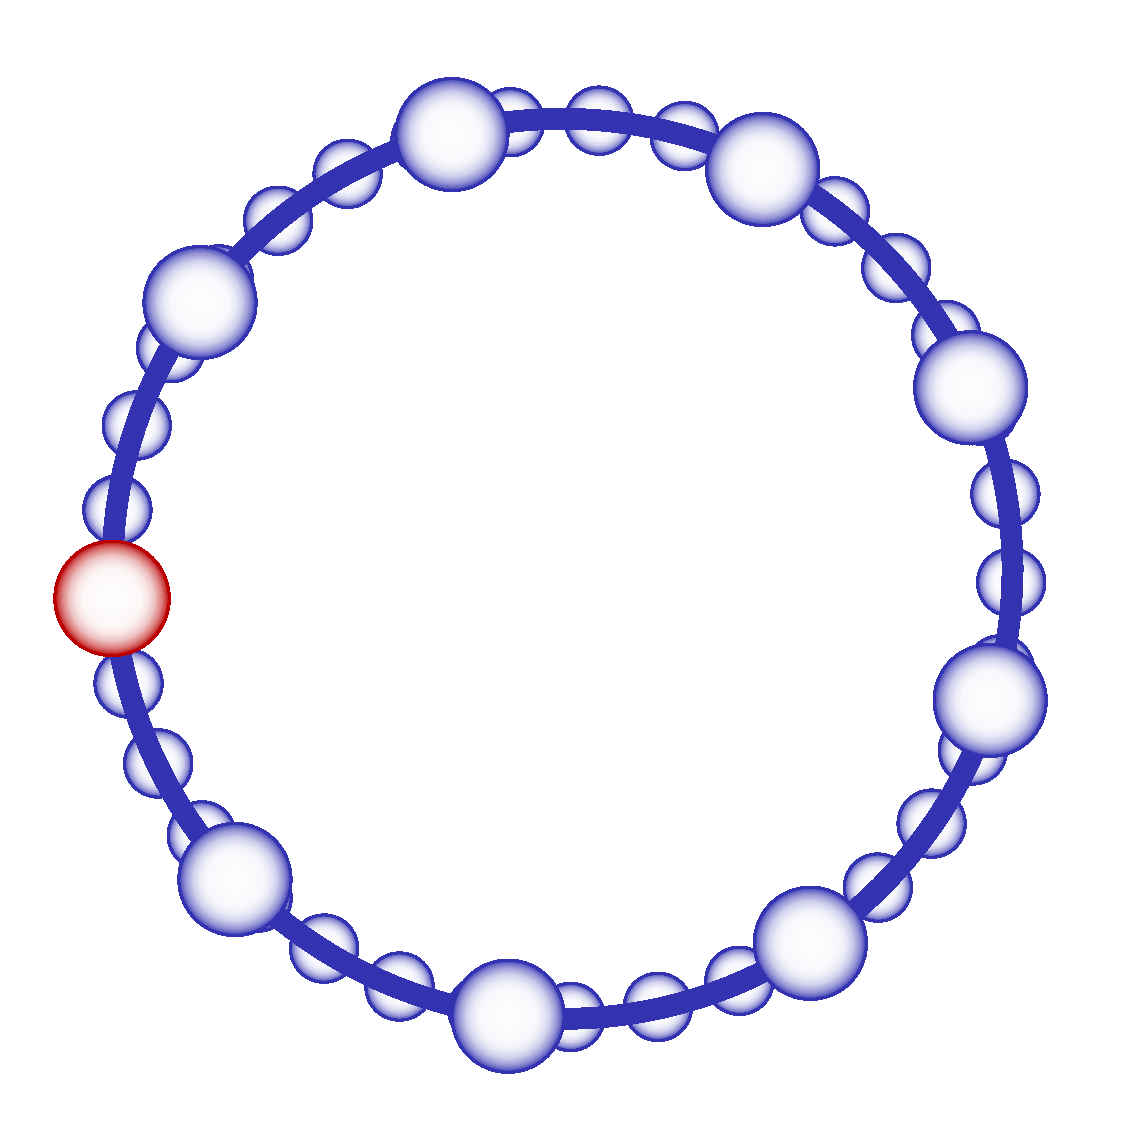
\includegraphics[width=6cm]{diagrams/ServiceHighlight}
        \end{overlayarea}
    \end{center}
    \end{columns}
\end{frame}

\begin{frame}
    \frametitle{Routing Information}

    \begin{columns}

    \column{5.5cm}
    \begin{overlayarea}{\textwidth}{1\textheight}
    Stealth Node ID = 3284...

    \begin{itemize}
        \item{Routing table}
        \begin{itemize}
            \item{Single row}
            \item{Extra entry}
%           \item{\footnotesize 97\% of time first row is used}
%            \item{\footnotesize Better than random first hops}
        \end{itemize}
    \end{itemize}

    \rowcolors[\hline]{1}{blue!20}{blue!10}
    \begin{tabular}{l!{\vrule}c c c c c c}
    \hline
      & 0 & 1 & 2 & 3 & ... & f\\
    0 & x & x & x & x & ... & x\\
    \end{tabular}

    ~\\
    \begin{itemize}
        \item{No Leafset}
    \end{itemize}

    \end{overlayarea}

    \column{5.5cm}
    \begin{center}
        \begin{overlayarea}{\textwidth}{\textheight}
            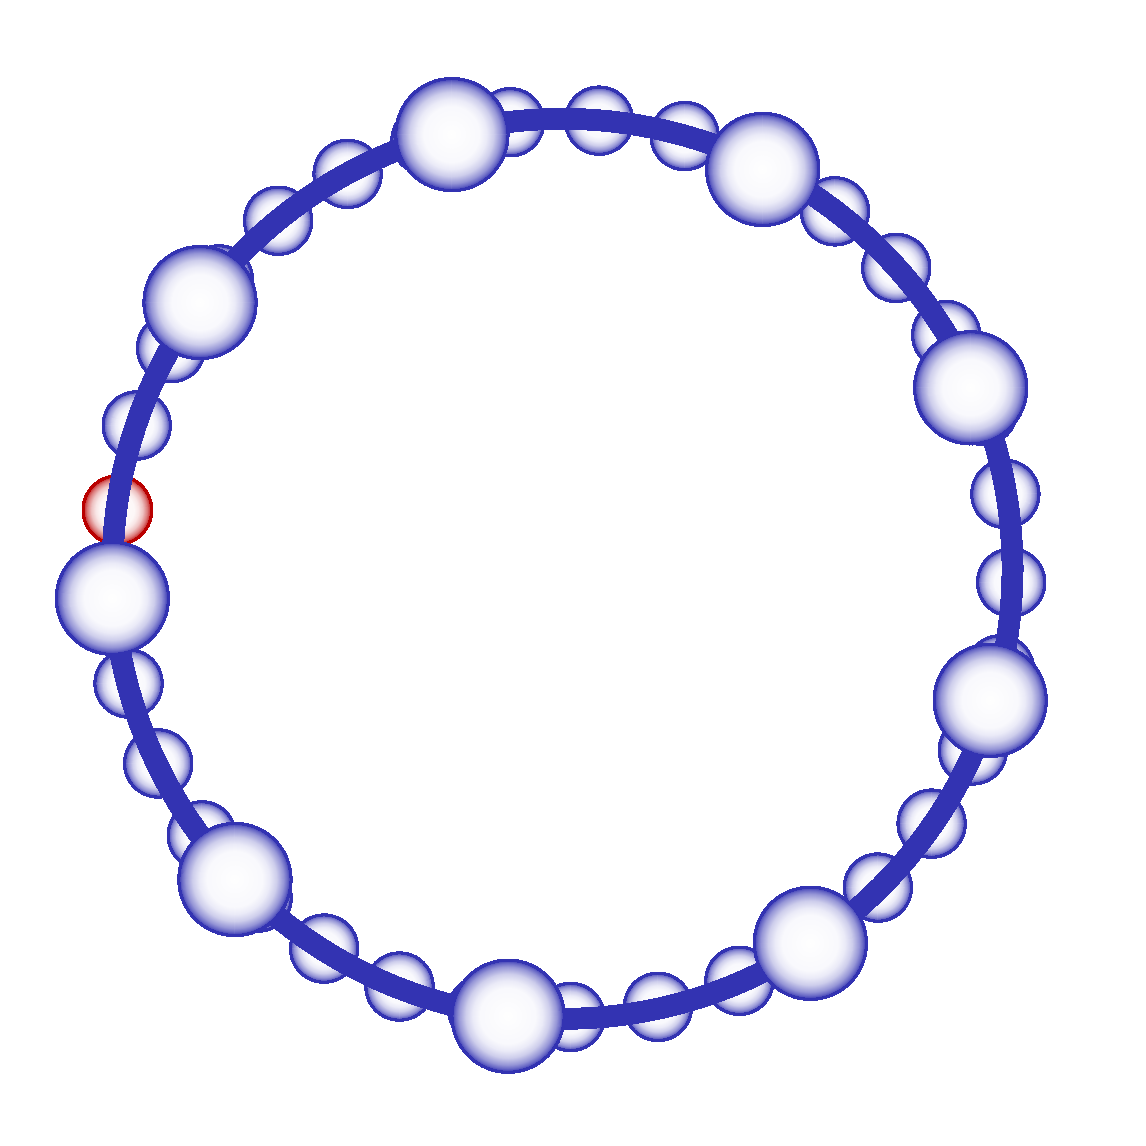
\includegraphics[width=6cm]{diagrams/StealthHighlight}
        \end{overlayarea}
    \end{center}

    \end{columns}
\end{frame}


\section{Models for Perfect Routing}

\subsection{Markov Chain}
\begin{frame}
\frametitle{Models for Pastry and Stealth DHT}
   \begin{itemize}
   \item  \textbf{Compute Expressions for Expected Number of Lookup Hops}
   \begin{itemize}
        \item  Using Discrete Markov  Chains
   \end{itemize}
   \vspace{+0.15in}
   \item  \textbf{Perfect Routing}
        \begin{itemize}
             \item All entries in  routing tables exist
             \item Not realistic!
         \end{itemize} \vspace{+0.15in}
    \item  \textbf{Imperfect Routing}
         \begin{itemize}
             \item Some entries are empty
         \end{itemize}
    \end{itemize}
\end{frame}

\subsection{Discrete Markov Chain}
\begin{frame}
\frametitle{Discrete Markov Chain}
   \begin{itemize} \vspace{-0.3in}
    \item{\textbf{Routing States}}
        \begin{itemize}
          \item[]
          \item $X_n \in \{0,1,2,\cdots,h,h+1\}$
          \item $X_n = 0 \rightarrow$ Source State
          \item $X_n = h+1 \rightarrow$ Destination state \vspace{+0.05in}
          \item [] %$h = log_{2^b} N$: maximum number of hops for perfect routing,
        \end{itemize} \vspace{0.1in}
    \item{\textbf{Transitions}}
        \begin{itemize}
           \item[]
           \item  $P(X_n  = j / X_n = i) = p_{ji}$
           \item  Transitions due to \textbf{Routing Table} or \textbf{NodeIDs}
           \item  \textbf{Hop} transitions, \textbf{non-Hop} transitions
        \end{itemize}
    \end{itemize}
\end{frame}

\begin{frame}
\frametitle{Prefix Match Probabilities} \vspace{-0.15in}
   \begin{itemize}
%     \item \textbf{Routing on DHT} \\
%         ~~~~Based on prefix match to identify  next hop  \\
%     \vspace{+0.05in}
     \item \textbf{Prefix Match probabilities} \\Node IDs and keys are  $2^b$
     entries long.  Let $L$ be the prefix match length, then
       \vspace{-0.2in}
     \item[]\begin{eqnarray}
                \nonumber p  &=&  P(L = 1) ~~~~ = 1/2^b \\
                \nonumber q  &=&  P(L=0) ~~~~ = 1- 1/2^b
             \end{eqnarray}
     \item[] Thus,   $P(L = i) = p^i$
    \item []
    \item \textbf{State Transitions in Markov Chains}\\
            ~~~~Based on prefix match
   \end{itemize}
\end{frame}

\subsection{Transition probabilities}
%\subsection{}
\begin{frame}
\begin{block}{$X_n = 0$}
\begin{center}
    \begin{figure}%{\textwidth}{0.2\textheight}
        \includegraphics<1>[width=7cm]{slides/First.pdf}
    \end{figure}
\end{center}
\end{block}

\begin{block}{}
   \begin{itemize}
            \item \textbf{$p_{i0} = P(X_n = i/X_n = 0)$,~~~$\forall i >
            0$}
                        \item[] %Transitions from state $0$ dont represent hops
             \item The node has a key to lookup for
                 \begin{itemize}
                    \item[] %No prefix match, $\implies p_{10} = q$
                    \item[]
                 \end{itemize}
    \end{itemize}
\end{block}
\end{frame}

%\subsection{Transition probabilities:  $p_{ji}$}
%\subsection{}
\begin{frame}
\begin{block}{$X_n = 0$}
\begin{center}
    \begin{figure}%{\textwidth}{0.2\textheight}
        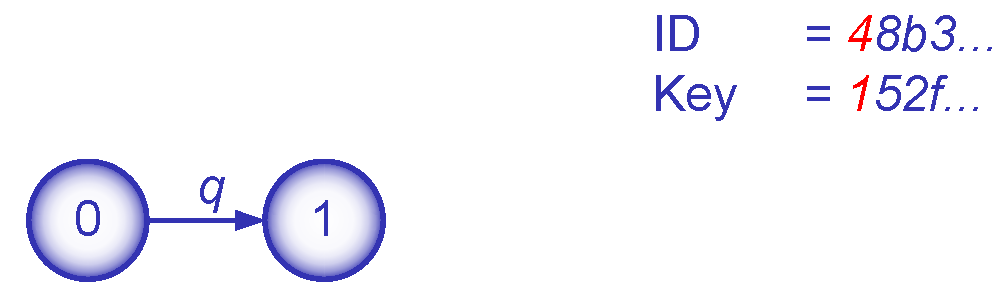
\includegraphics[width=7cm]{slides/Second-1.pdf}
    \end{figure}
\end{center}
\end{block}

\begin{block}{}
   \begin{itemize}
            \item[] %\textbf{$p_{i0} = P(X_n = i/X_n = 0)$,~~~$\forall i > 0$}
            \item No prefix match, $\implies p_{10} = q$ %The node has a key to lookup for
                 \begin{itemize}
                    \item[]% No prefix match, $\implies p_{10} = q$
                    \item[]
                 \end{itemize}
            \item[] %Transitions from state $0$ dont represent hops
    \end{itemize}
\end{block}
\end{frame}

\begin{frame}
\begin{block}{$X_n = 0$}
\begin{center}
    \begin{figure}%{\textwidth}{0.2\textheight}
        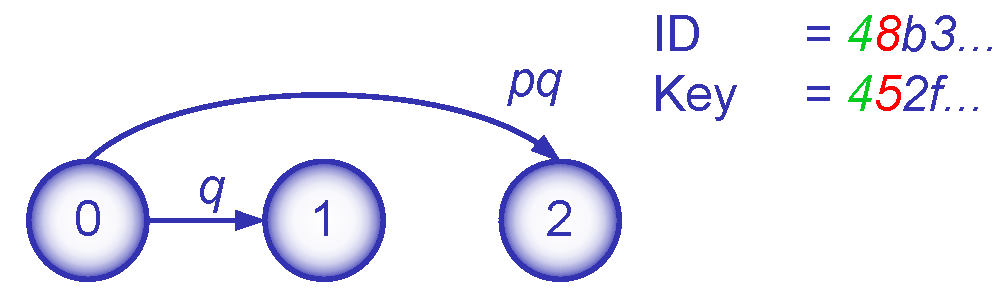
\includegraphics[width=7cm]{slides/Second-2.pdf}
    \end{figure}
\end{center}
\end{block}

\begin{block}{}
   \begin{itemize}
            \item[] %\textbf{$ p_{i0} = P(X_n = i/X_n = 0)$,~~~$\forall i > 0$}
            \item One prefix match, $\implies p_{20} = pq$ %The node has a key to lookup for
                 \begin{itemize}
                    \item[] %One prefix match, $\implies p_{20} = pq$
                    \item[]
                 \end{itemize}
            \item[] %Transitions from state $0$ dont represent hops
    \end{itemize}
\end{block}
\end{frame}


\begin{frame}
\begin{block}{$X_n = 0$}
\begin{center}
    \begin{figure}%{\textwidth}{0.2\textheight}
        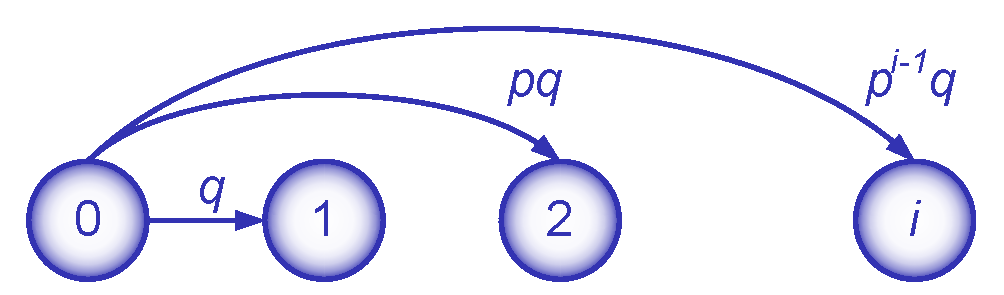
\includegraphics[width=7cm]{slides/Second-3.pdf}
    \end{figure}
\end{center}
\end{block}

\begin{block}{}
   \begin{itemize}
            \item[] %\textbf{$ p_{i0} = P(X_n = i/X_n = 0)$,~~~$\forall i >  0$}
            \item At least one prefix match, $\implies p_{i0} = p^{i-1}q$, $i\ge 1$ %The node has a key to lookup for
                 \begin{itemize}
                    \item[] %At least one prefix match, $\implies p_{i0} = p^{i-1}q$, $i\ge 1$
                    \item[]
                 \end{itemize}
            \item Transitions from state $0$ dont represent hops
    \end{itemize}
\end{block}
\end{frame}

\begin{frame}
%\frametitle{State ($X_n= i$)}
\begin{block}{$X_n= i$}
  \begin{center}
    \begin{figure}%{\textwidth}{0.2\textheight}
        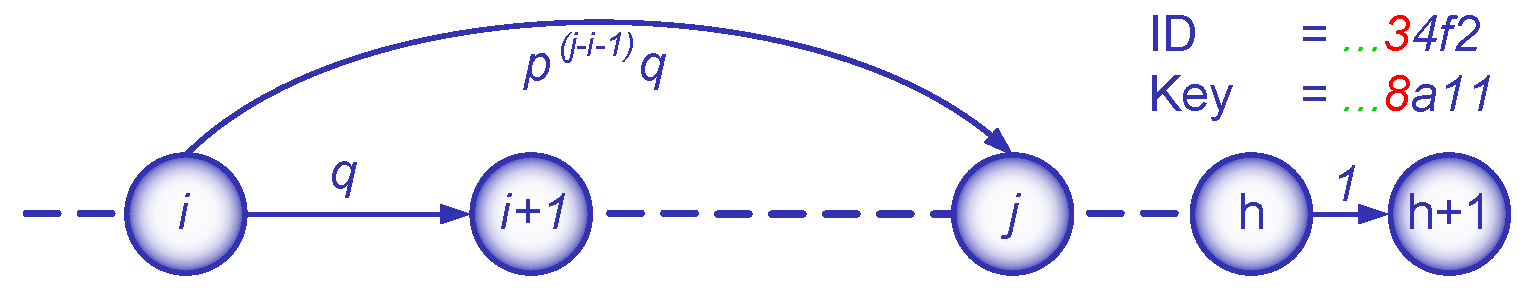
\includegraphics[width=8cm]{slides/Third-1.pdf}
    \end{figure}
  \end{center}
\end{block}
\begin{block}{}
   \begin{itemize}
   \item \textbf{$p_{ji} = P(X_n = j/X_n = i)$}
 %\begin{itemize}
 %\item  $p_{i+1,i} =$ probability that Node ID doesn't improve the prefix
 % match
% \end{itemize}
 %   \item \textbf{$p_{ji} = P(X_n = j/X_n = i)$}
     \begin{itemize}
     \item[] \[ p_{ji} = \left\{ \begin{array}{ll}
         0 & \mbox{if $j \le i$}\\
         p^{j-i-1}q & \mbox{if $i < j \le h$} \\
         1   &  \mbox{if $i = h$, $j=h+1$}
         .\end{array} \right. \]
     \end{itemize}
   \end{itemize}
   \end{block}
\end{frame}


%\subsection{Transition Probabilities}

\begin{frame}
\frametitle{Stealth DHT}
\begin{block}{$X_n= 0$}
   \begin{itemize}
        \item Probabilities for service nodes are the same as for Pastry
        nodes
        \item Stealth nodes have 1-row routing tables
        \item[]~~~~~Thus, $p_{10} = 1$
   \end{itemize}
\end{block}
\begin{block}{}
  \begin{center}
    \begin{figure}%{\textwidth}{0.2\textheight}
        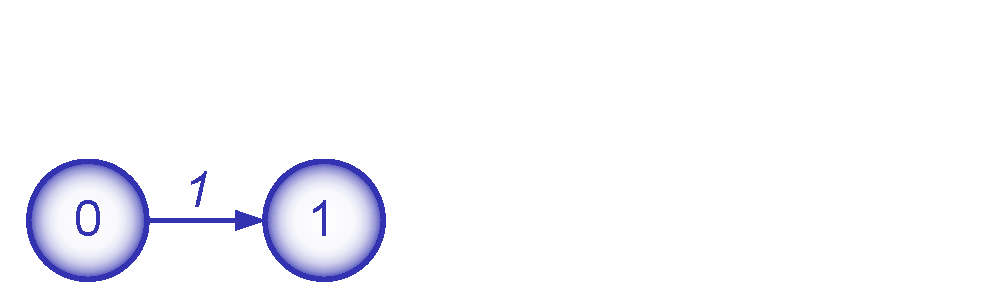
\includegraphics[width=7cm]{slides/Zero.pdf}
    \end{figure}
  \end{center}
\end{block}
\end{frame}


%\subsection{Transition Probabilities}
\begin{frame}
\frametitle{Markov Chains}
\begin{block}{Pastry; \textbf{$h = log_{2^b}N$}}
  \begin{center}
    \begin{figure}%{\textwidth}{0.2\textheight}
        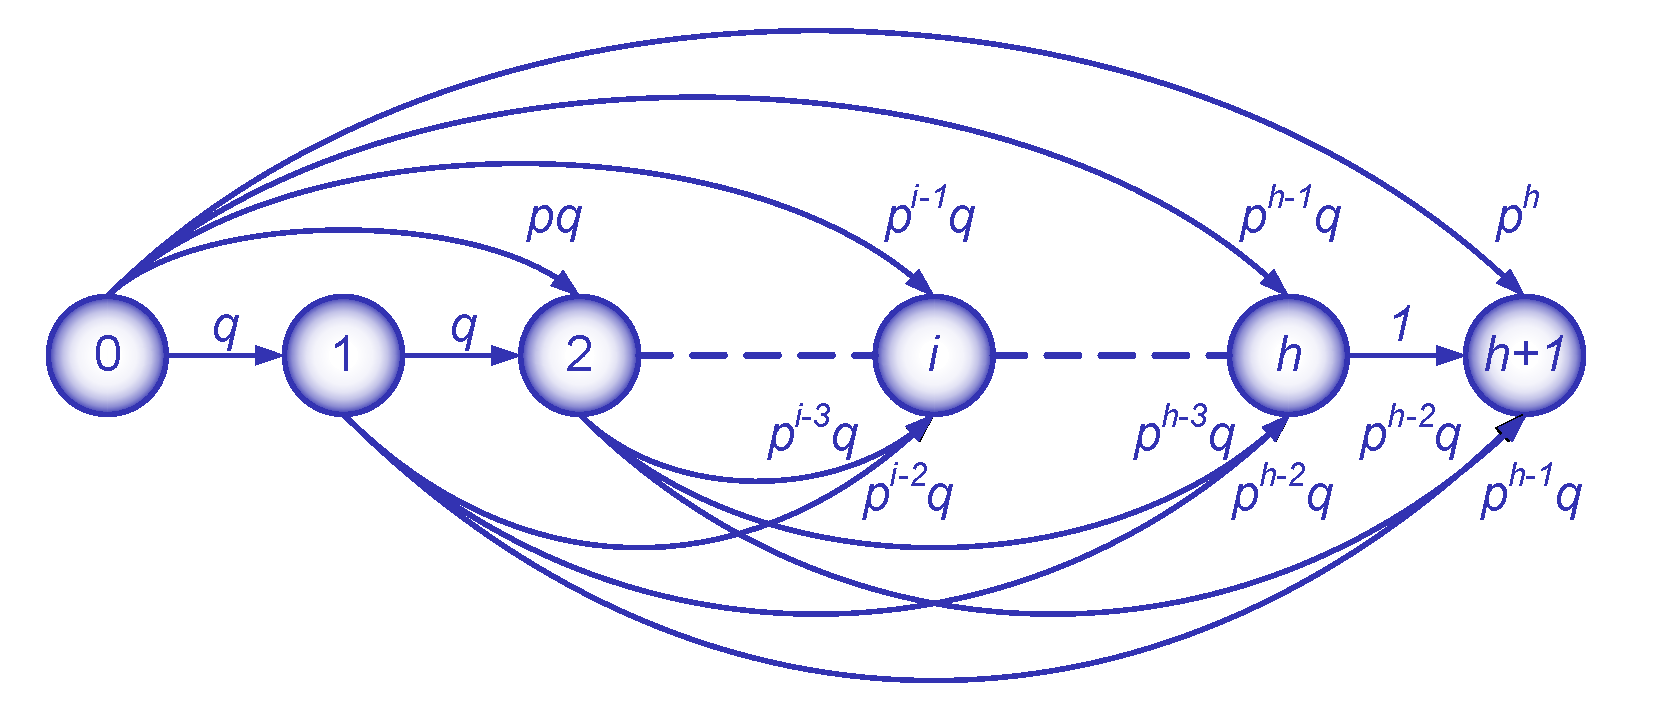
\includegraphics[width=6cm]{slides/Markov-NoFail}
    \end{figure}
  \end{center}
\end{block}
\begin{block}{Stealth DHT: \textbf{$h = log_{2^b}rN$}}
  \begin{center}
    \begin{figure}%{\textwidth}{0.2\textheight}
        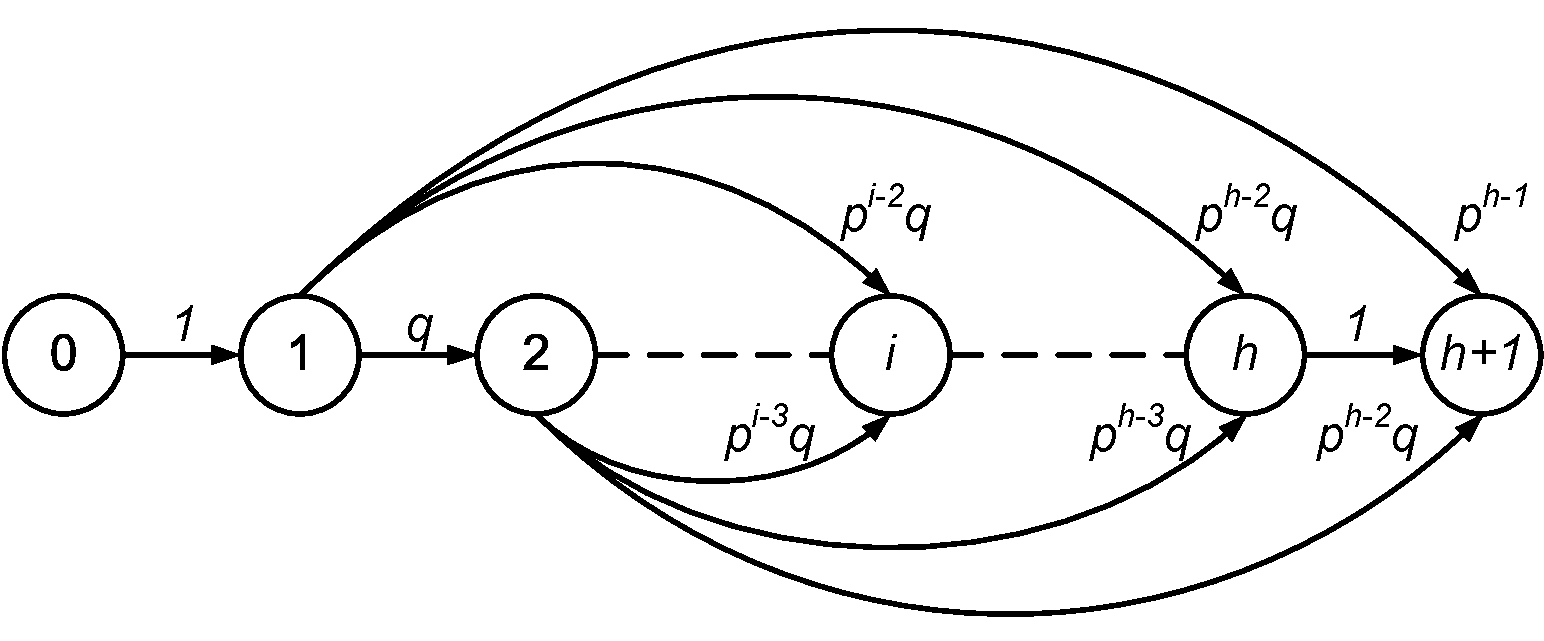
\includegraphics[width=6cm]{slides/Markov-SDHT-NoFail}
    \end{figure}
  \end{center}
\end{block}
\end{frame}


%\section{Expected number of hops}
%\subsection{Stationary solutions}
\begin{frame}
\frametitle{Stationary solutions}

   \begin{itemize}
        \item Irreducible, aperiodic
        \item We add a sure transition from from state $h+1$ to $0$,
        i.e., $p_{0,h+1}=1$
    \end{itemize}

    \begin{center}
    \begin{figure}%{\textwidth}{0.2\textheight}
        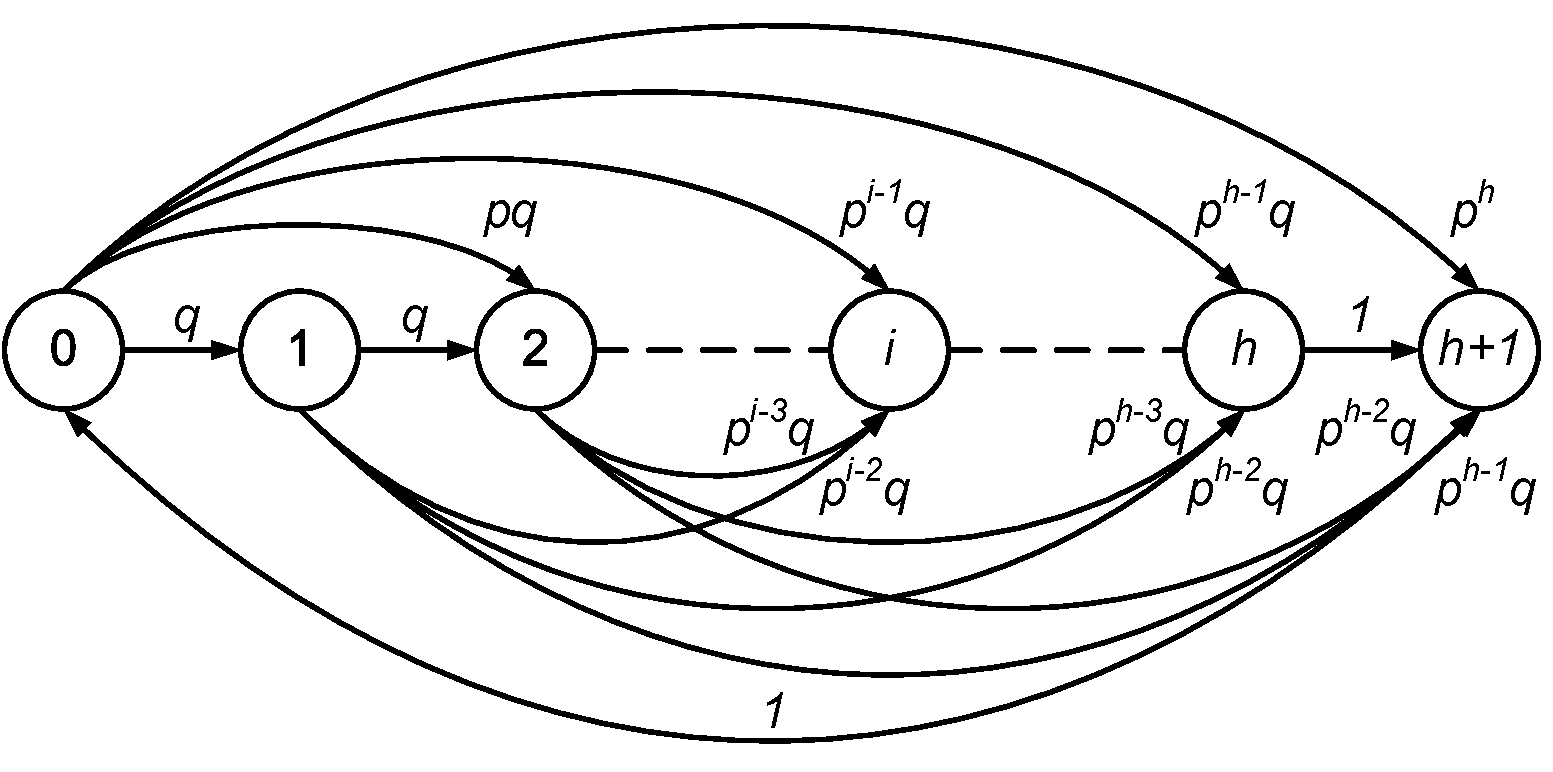
\includegraphics[width=8cm]{slides/Markov-Modify}
    \end{figure}
  \end{center}

\end{frame}


%\subsection{Expected number of hops}
\begin{frame}
\frametitle{Results}
   \begin{itemize}
    \item Perfect Routing Models  \vspace{+0.2in}
      \begin{itemize}
        \item {\Large \textbf{$H_{Pastry} = hq$}}, \\ \vspace{+0.1in} where $h = log_{2^b}
        N$ \vspace{+0.3in}
        \item {\Large \textbf{$H_{SDHT} =  (h-1)q+1$}}, \\ \vspace{+0.1in} where
        $h = log_{2^b}rN$, and $r$ is the fraction of service nodes
      \end{itemize}
  \end{itemize}
\end{frame}


\section{Models for Imperfect Routing}
\begin{frame}
\frametitle{Transition probabilities}
\begin{block}{}
  \begin{itemize}
    \item Definitions
    \begin{itemize}
      \item Let the probability of   an empty entry  be  $p_f$, then
      \item $q_f = 1-p_f$ is the probability of an entry  being not empty
   \end{itemize} \vspace{+0.15in}
   \item Transition probabilities
   \begin{itemize}
     \item No failures at state $0$, and state $h+1$
   \end{itemize}
  \end{itemize}
  \end{block}
\begin{block}{}
  \begin{center}
    \begin{figure}%{\textwidth}{0.2\textheight}
        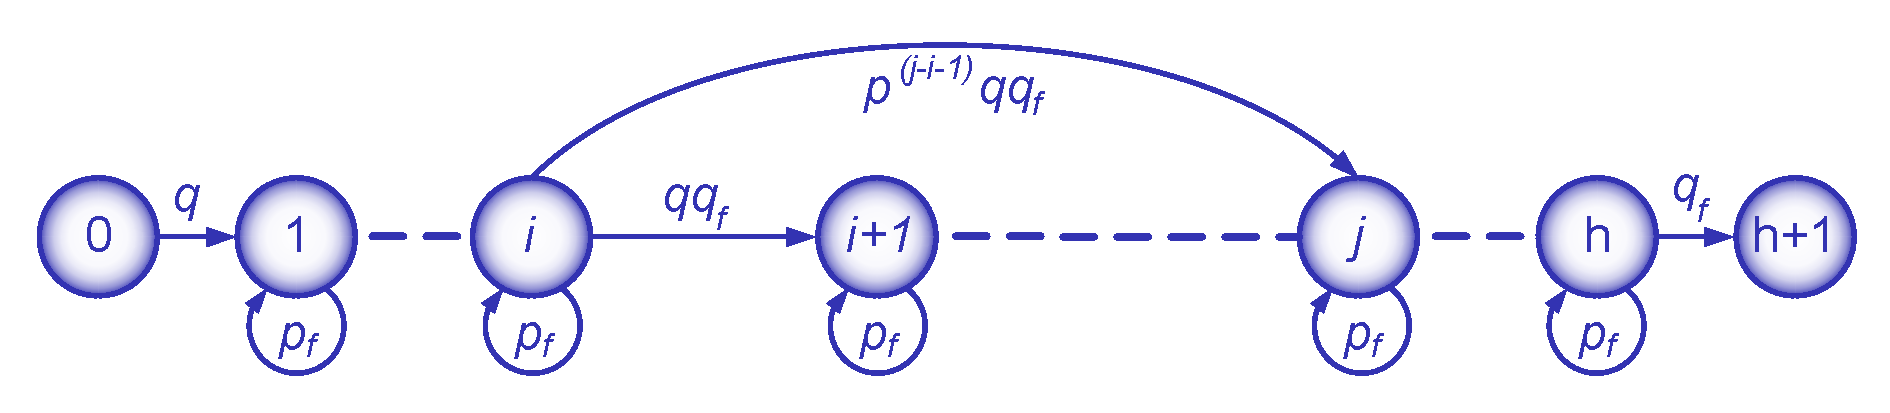
\includegraphics[width=10cm]{slides/Third-2.pdf}
    \end{figure}
  \end{center}
\end{block}
\end{frame}


\begin{frame}
\frametitle{Results}
   \begin{itemize}
    \item Imperfect Routing Models  \vspace{+0.2in}
      \begin{itemize}
        \item {\Large \textbf{$H^f_{Pastry} = \frac{hq}{q_f}$}}, \\ \vspace{+0.1in} where $h = log_{2^b}
        N$ \vspace{+0.3in}
        \item {\Large \textbf{$H^f_{SDHT} =  \frac{(h-1)q+1}{q_f}$}}, \\ \vspace{+0.1in} where
        $h = log_{2^b}rN$, and $r$ is the fraction of service nodes
      \end{itemize}
  \end{itemize}
\end{frame}


\section{Validation}
\subsection{Perfect Routing}
\begin{frame}
   \frametitle{Pastry}
  \begin{center}
    \begin{figure}%{\textwidth}{0.2\textheight}
        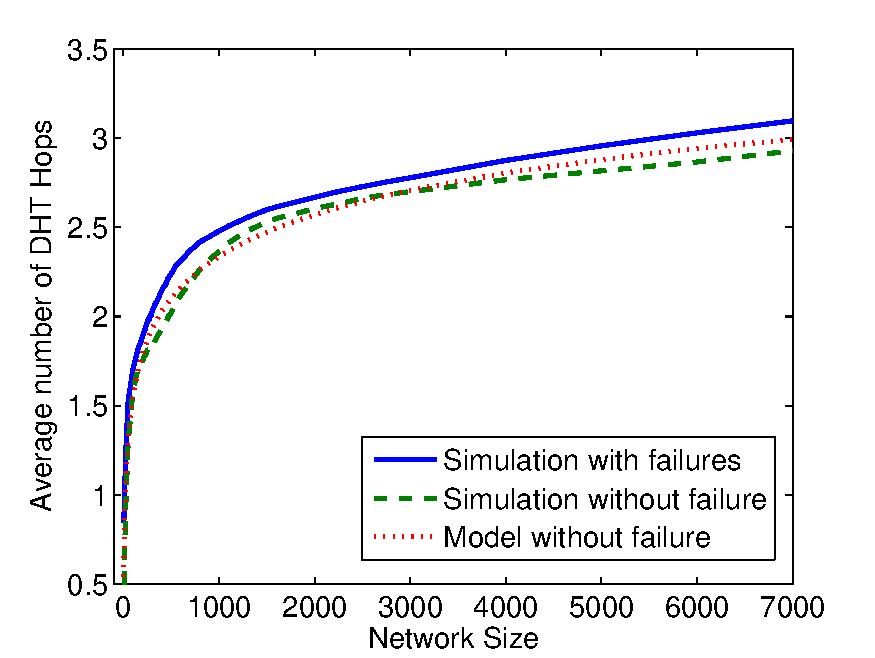
\includegraphics[width=7cm]{pdfplots/val_past1.pdf}
    \end{figure} \end{center}
\end{frame}

\subsection{Imperfect Routing}
\begin{frame}
   \frametitle{Pastry}
  \begin{center}
    \begin{figure}%{\textwidth}{0.2\textheight}
       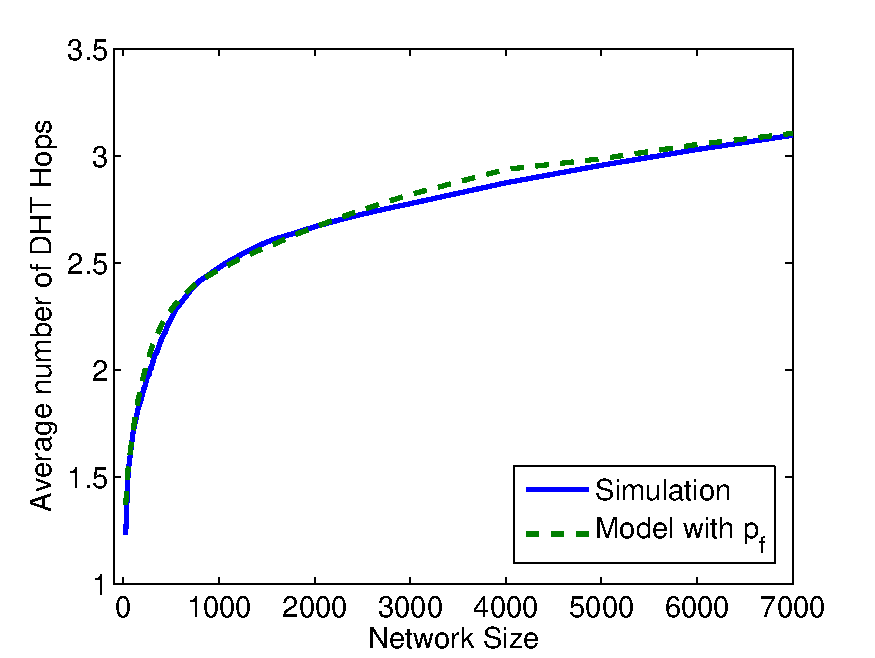
\includegraphics[width=7cm]{pdfplots/val_past2.pdf}
    \end{figure} \end{center}
\end{frame}

\begin{frame}
   \frametitle{Stealth DHT}
  \begin{center}
    \begin{figure}%{\textwidth}{0.2\textheight}
        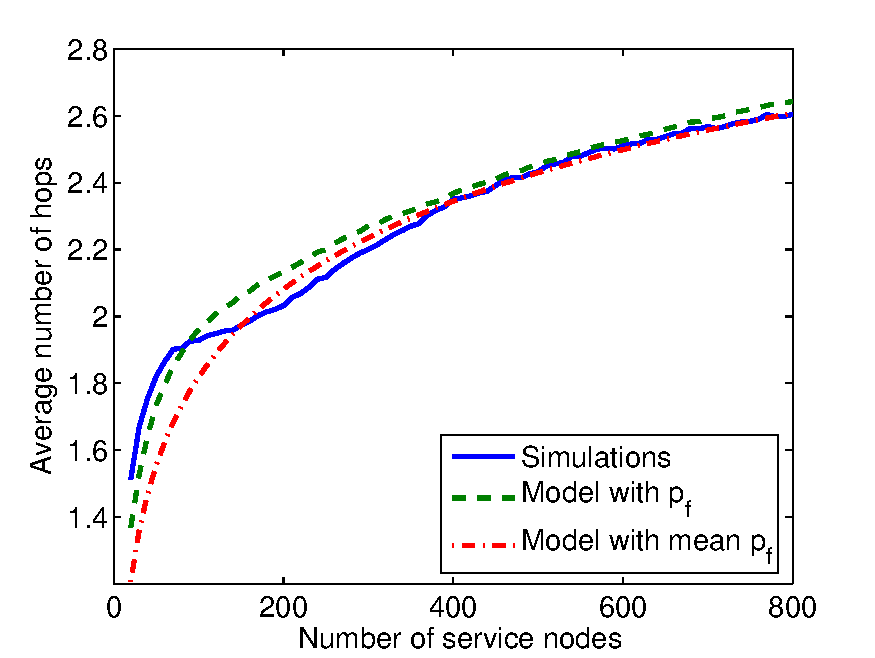
\includegraphics[width=7cm]{pdfplots/val_stealth1.pdf}
    \end{figure} \end{center}
\end{frame}


% results section

\subsection{Conclusion}
\begin{frame}
    \frametitle{Conclusion}
    \vspace{-0.5in}
        \begin{itemize}
            \item{The derived models are  well \textbf{validated} by simulations}
            \item{They can be used to \textbf{quickly} analyze the protocols, instead of simulations}
        \end{itemize}
\vspace{0.2in}
       \textbf{ Related Papers}
         \begin{itemize}
            \item  \textbf{BaRT} and \textbf{Koorde}, by \textbf{Spognardi} et al, In
                   Hot-P2P 2006.
            \item  Google \emph{Stealth DHT}
         \end{itemize}

\end{frame}


\begin{frame}
  %\frametitle{Thank you for listening}
  \begin{center}
    \textbf{Thank you for listening\\
    Any questions?\\}
    \titlepage
  \end{center}
\end{frame}

\end{document}
